\documentclass[11pt, titlepage, a4paper]{scrartcl}
\usepackage[utf8]{inputenc}
\usepackage{csquotes} 
\usepackage{amsmath}
\usepackage{graphicx}
\usepackage{authblk}
\usepackage[T1]{fontenc}
\usepackage{lmodern} % Improved font rendering
\usepackage[a4paper]{geometry}
\usepackage[hidelinks]{hyperref}
\usepackage[english]{babel}
\usepackage{lineno}
\usepackage{pgfgantt}
\usepackage{xcolor}
\usepackage{enumitem}
\usepackage{cleveref}
\usepackage{pdflscape}
\usepackage{amsmath}
\usepackage{array}
\usepackage[acronym]{glossaries}

\usepackage{appendix}
\usepackage[backend=biber, style=ieee, sorting=none, url=true]{biblatex}
\addbibresource{proposal.bib} % Imports bibliography file

% Customize URL appearance
%\urlstyle{same} % Keeps the URL in the same font as the main text
\hypersetup{
    breaklinks=true
}

\title{Visualizing Wind Energy: Digital Twins as Tools for Public Engagement}
\author{Emily Sterthaus \\ Matriculation Number: 451 342 \\ \href{mailto:m_ster15@uni-muenster.de}{m\_ster15@uni-muenster.de}}
\affil{Institute of Geoinformatics, University of Münster}
\date{\today}

\geometry{
    a4paper,
    left=2.5cm,
    right=2.5cm,
    top=2.5cm,
    bottom=2.5cm
}


\definecolor{barblue}{RGB}{153,204,255}
\definecolor{groupblue}{RGB}{51,102,254}
\definecolor{linkred}{RGB}{165,0,33}

\newlist{questions}{enumerate}{2}
\setlist[questions,1]{label=RQ\arabic*.,ref=RQ\arabic*}
\setlist[questions,2]{label=(\alph*),ref=\thequestionsi(\alph*)}

% Customizing cref format
\crefformat{questionsi}{#2#1#3}
\crefformat{questionsii}{#2#1#3}


\makeglossaries
\newacronym{i3s}{I3S}{Indexed 3D Scene Layer}
\newacronym{nrw}{NRW}{North Rhine-Westphalia}
\newacronym{ogc}{OGC}{Open Geospatial Consortium}
\newacronym{epsg}{ESPG}{European Petroleum Survey Group}
\newacronym{fme}{FME}{Feature Manipulation Engine}

\begin{document}

\maketitle


\newpage
\tableofcontents
\newpage
\begin{linenumbers}
    \section{Introduction}
    The siting of wind turbines is a multifaceted issue, fraught with complexity and political nuances. Onshore
    turbine placement is governed by a myriad of regulations, e.g., in Lower Saxony incorporating a range of parameters including, but not
    limited to: minimum distance to residential buildings, the foundation may only stand on a parcel of land and the
    turbines need a minimum distance between each other
    \cite{niedersachsischesministeriumfurumweltenergieundklimaschutzPlanungUndGenehmigung2021}.

    However, the public perception of wind turbines is often negative, with many people citing noise pollution, visual impact as reason for their opposition to wind power plants. This is despite the fact that wind power is a clean, renewable energy source that can help to reduce greenhouse gas emissions and combat climate change.

    This leads to a situation where the siting of wind turbines is often met with resistance from local communities, who may be concerned about the impact of the turbines on their quality of life. Which makes it a heavy politicized issue, with local governments often facing opposition from residents when trying to approve new wind power projects \cite{kwasniewskiWindenergieVerhindertAntiWindkraftBewegung2021}.

    \section{Background and Literature Review}
    \subsection{Digital Twins}
    The concept of digital twins, first introduced in 2000, has gained significant popularity in recent years. Originally, a digital twin was defined as an exact mirror image of the real world, replicating all elements and processes. However, the definition has since broadened. Currently, a digital twin is understood as a simulation model that operates alongside real-time processes, applicable not only to physical systems but also to social and economic systems. Thus, a digital twin serves as an abstraction or model of the real world \cite{battyDigitalTwins2018}.

    Digital twins have been adopted across various disciplines, including manufacturing, the automotive industry, and the energy sector, addressing different challenges within each field. As accurate replicas of the real world, they are particularly effective for integrating solutions into complex analyses and providing decision support \cite{pylianidisIntroducingDigitalTwins2021}.

    \subsection{Technical Aspects}
    A fundamental aspect of this thesis is the utilization of 3D Meshes, specifically \gls{ogc} \gls{i3s} meshes. The \gls{i3s} format facilitates the streaming and distribution of 3D content across various (enterprise) systems. A single \gls{i3s} dataset, referred to as a scene layer, serves as a container for extensive and diverse 3D geographic data. To fully define a scene layer, both a layer type and a layer profile are required.
    The \gls{i3s} format supports various data types, including 3D objects, integrated meshes, point clouds, and building scene layers. It is designed with web, mobile, and cloud use cases in mind. Although it is developed by Esri, it is also part of the \gls{ogc} standards \cite{esriincI3sspec}.

    Given that map.apps is based on Esri's ArcGIS Maps SDK for JavaScript, integrating an \gls{i3s} layer into the application is straightforward. The ArcGIS Maps SDK for JavaScript also provides additional analysis tools when an ArcGIS Enterprise environment is available. Particularly relevant to this project are the shadow analysis \cite{esriincShadowCast} and viewshed analysis tools \cite{esriincGeoprocessingViewshedAnalysis}.

    \subsection{Wind Energy}
    As climate change becomes an increasingly pressing issue, the importance of renewable energy sources continues to grow. The European Union aims to achieve carbon neutrality by 2050, with renewable energy playing a crucial role in reaching this objective \cite{europeancommission.directorategeneralforclimateaction.GoingClimateneutral20502019}. Wind turbines present a viable solution, as they are a clean and renewable energy source with negligible greenhouse gas emissions \cite{pryorClimateChangeImpacts2020}.

    Germany, in particular, aims to significantly increase its share of renewable energy. A spatial strategy involves allocating 2\% of the land area for wind energy, with the objective of producing 115 GW of wind energy by the end of 2030 \cite{WindenergieLand}.


    In \gls{nrw}, the "Windenergieerlass" (Wind Energy Decree) \cite{nrwErlassFurPlanung} regulates the allocation of wind turbines. This administrative regulation aims to balance the planning of wind turbines with considerations for residents and environmental protection \cite{nrwErlassFurPlanung}.

    Despite the challenges associated with the placement of wind turbines due to local community concerns, a recent survey revealed that onshore wind turbines are widely accepted across Germany, with over 81\% approval. Additionally, local community acceptance for existing wind turbines is high, with approval rates exceeding 80\%. The survey also indicates that the acceptance of existing wind turbines is higher than that of planned ones \cite{fachagenturwindenergieanlandUmfrageZurAkzeptanz}.

    \subsection{con terra Affiliations \gls{nrw}}
    %Ich bin mir nicht sicher ob das hier sein muss. Holger wollte das haben aber ich weiß nicht ganz was da rein muss... 
    In addition to various other projects within \gls{nrw}, con terra is currently engaged in a digital twin project aimed at enhancing hazard defense mechanisms in the \gls{nrw}. As part of this initiative, con terra has access to several high-quality datasets, including the comprehensive \gls{i3s} Mesh for \gls{nrw}.


    \section{Research Question}

    This study aims to address one primary research question:

    \begin{questions}
        \item \label{rq:first_q} How effectively does the implemented digital twin interface enable non-expert users to accurately interpret and manipulate key wind energy parameters?

    \end{questions}

    To specify \ref{rq:first_q}, the following sub-questions are defined:

    \begin{itemize}[label={--}]
        \item To what extent can users accurately interpret the visual impairement simulations provided by the digital twin?
        \item How successfully do users navigate and apply the legal restrictions for turbine placement using the interface?
        \item What level of understanding do users demonstrate regarding the trade-offs between energy output and environmental impact as presented in the digital twin?
    \end{itemize}

    The primary objective of \ref{rq:first_q} is to assess the interaction between non-expert users and the digital twin. Following an experimental research approach, the evaluation will focus on the usability of the digital twin, with a specific emphasis on the ease with which users can interact with and comprehend the application. Consequently, the focus will be solely on the interaction with the digital twin.

    For \ref{rq:first_q}, there will be no null or alternative hypothesis, as this follows a more exploratory approach.

    Additionally, there will be a comparative study about how the digital twin compares to traditional methods of public engagement.


    \section{Objectives}
    \subsection{General Objective}
    The objective of this research is to explore the potential of digital twins to impact public opinion regarding wind energy installations. The project involves the development of a digital twin for a wind power facility to accurately simulate and visualize its environmental effects. This research is designed to provide stakeholders with a detailed assessment of both the benefits and limitations associated with wind turbines, thereby aiding in the decision-making process for future developments.

    A digital twin is conceived as an interactive 3D application that allows users to traverse a specified test area, install turbines, and observe their influence on the local environment. The application is equipped to simulate aspects such as noise pollution and visual impacts, which include changes in the landscape and shadow effects caused by the turbines.

    %Additionally, the digital twin will evaluate the risk of bird strikes and analyze the energy output and potential savings over determined periods. 
    % Wurde entfernt aufgrund holgers feedback, bin mir nicht sicher wie ich das  einbauen soll
    It will include a feature to ensure that turbine placements comply with existing legal frameworks and zoning regulations.

    Technologically, the digital twin will integrate various datasets to enhance its realism and functionality. It will support \gls{ogc}/Esri \gls{i3s} Meshes \cite{esriincI3sspec}, incorporate weather data from DWD, and use land use classifications from local planning documents % (FNP? Bebauungsplan?)
    to ensure optimal turbine placement based on environmental and regulatory considerations. The application will also provide a comprehensive selection of turbine models, enabling stakeholders to choose configurations that best fit their requirements.

    An extensive user study will be conducted to evaluate the usability of the digital twin, focusing on the ease with which users can interact with and understand the application.





    \subsection{SMART Objectives}
    As the goals beforehand describe the general objective of the thesis, the SMART objectives will describe the specific goals of the thesis. The SMART objectives are as follows:
    \begin{itemize}[label={--}]
        \item Develop a digital twin interactive 3D application  that allows users to navigate a specific test area and place turbines to assess their visual and noise impact on the surroundings.
        \item Implement a feature  in the digital twin to simulate the visual impact caused by wind turbines, including shadow casting and changes to the landscape.
        \item Introduce a noise pollution simulation within the digital twin to quantify the acoustic impact of wind turbines at various distances and under different weather conditions.
        \item Integrate an energy analysis tool into the digital twin  that calculates real-time energy generation and potential energy savings from placed turbines over specified periods.
        \item Incorporate a legal assessment tool  in the digital twin to verify turbine placements against local regulations and zoning requirements.
        \item Support \gls{ogc}/Esri \gls{i3s} Meshes for realistic terrain modeling, providing a detailed and accurate representation of the test area.
        \item Integrate weather data from DWD into the digital twin.
        \item Incorporate land use classifications from local plans into the digital twin by to ensure the placement of turbines is optimized according to zoning regulations and environmental suitability.
        \item Provide a comprehensive catalog of turbine models, to allow stakeholders to choose from various options based on their specifications and needs.
        \item Develop and integrate a module for evaluating inter-turbine interactions, such as wake steering, into the digital twin \cite{howlandWindFarmPower2019a}.
        \item  Design and implement a user-friendly interface for the digital twin, focusing on intuitive navigation and interaction to ensure that stakeholders can effectively utilize the application without prior technical expertise.
        \item Conduct a comprehensive user study to evaluate the usability of the digital twin prototype. This study will assess participants' ease of understanding and interacting with the application, aiming to confirm that the interface and functionalities are intuitively designed.
    \end{itemize}


    \section{Methodology}
    The methodology for this research project will involve a combination of data acquisition, software development, and user studies. The project will be divided into several phases, each focusing on a specific aspect of the digital twin development and evaluation process.

    \subsection{Data Acquisition}
    Data acquisition is a pivotal component in the development of the digital twin, necessitating a systematic approach to collate multifarious datasets. This approach ensures an encompassing environmental and regulatory context, essential for accurate simulation and analysis. The designated test area for data collection is \gls{nrw}, Germany. Choosing which part of \gls{nrw} to focus on will be determined by the availability of data and the feasibility of acquiring the necessary information.
    The following datasets will be acquired:

    \begin{itemize}
        \item \textbf{Terrain Data:} High-resolution terrain models are crucial for assessing site suitability and environmental impacts. We will utilize Esri \gls{i3s} Meshes, supplied by the \gls{nrw}, facilitated through a partnership with con terra.

        \item \textbf{Meteorological Data:} Specifically, wind data is integral for the site selection and optimization of wind turbine placements. This dataset will be sourced from the Deutscher Wetterdienst (DWD), which provides detailed wind statistics critical for wind energy applications in Germany \cite{deutscherwetterdienstWinddatenFurWindenergienutzer}.

        \item \textbf{Land Use Classifications and Zoning Information:} Essential for legal compliance and environmental planning, land use and zoning data will be sourced from the \gls{nrw} Data Portal \cite{ministeriumfurheimatkommunalesbauunddigitalisierungdeslandesnordrhein-westfalenOpenNRW}. This information facilitates the assessment of site suitability and regulatory alignment for wind turbine installation.

        \item \textbf{Wind Turbine Specifications:} Information regarding various wind turbine models will primarily be sourced from Enercon’s comprehensive product portfolio \cite{enerconglobalgmbhENERCONWindenergieanlagenPortfolio}. To ensure a broader representation of available technologies, additional inquiries may be made to other turbine manufacturers, thereby expanding our dataset with diverse turbine types and specifications.
    \end{itemize}

    Integration of these datasets into the digital twin is anticipated to be straightforward, leveraging the capabilities of map.apps within an ArcGIS Enterprise Environment, supported by the data transformation and integration functionalities of \gls{fme}.




    \subsection{Development}
    The digital twin will be developed as a map.apps application, leveraging its capabilities for interactive 3D application development. The selection of map.apps, a proprietary product developed by con terra, was driven by several factors. Primarily, its foundation on the ArcGIS JavaScript API offers significant advantages. This  enables the visualization of any 3D environment within local Coordinate Reference Systems, specifically \gls{epsg}: 3857, which is mandated by German law. Currently, other open-source tools, such as CesiumJS, do not support this capability. Furthermore, map.apps supports one of the common standards for 3D meshes, Esri/\gls{ogc}'s \gls{i3s}. While 3D tiles present an alternative to \gls{i3s}, within the map.apps environment, they do not offer any additional benefits. The primary development efforts will focus on the creation of isolated bundles, each tailored to specific functionalities required for the digital twin. These functionalities include a noise simulation, a visual impact simulation, an energy analysis tool, a legal assessment tool, an inter-turbine interaction module, and the user interface. The development will predominantly involve JavaScript/TypeScript, complemented by HTML and CSS for crafting the user interface. The principal frontend components will be designed as Vue components.

    The infrastructure necessary for this project, including the map.apps installation, ArcGIS Enterprise, \gls{fme}, and the required servers, will be provided by con terra.

    Should there be limitations in developing solely in JavaScript for the frontend, an additional Python component may be introduced to enable more advanced analysis capabilities.


    %Todo: Wie führt man eine User Study durch?
    %Todos: Studien Art? Gibt es eine kontrollgrupe? Wie sieht die studie aus? Wie viele teilnehmer? Wie werden die teilnehmer ausgewählt? Wie wird die studie ausgewertet?
    \subsection{User Study}
    As part of this thesis, a user study will be conducted to address the primary research question \cref{rq:first_q}. The study will be divided into two distinct parts. The first part will concentrate on evaluating the usability of the digital twin, assessing user comprehension and experience across all aspects of the digital twin.
    The study will not employ any specific selection criteria for participants. All participants will interact with an identical version of the digital twin system, without any randomization or variation in experimental conditions between subjects. There will be no designated control groups in this study design. As such, the sampling method employed in this study can be considered non-probabilistic sampling. To compensate for the limitations of this sampling method, demographic data will be collected from the participants. \cite{lazarResearchMethodsHuman2017}. The selection of participants would be likely to be convenience sampling from colleagues at con terra and other students.
    The study will involve a maximum of five participants, as it is suggested that five individuals can identify 80\% of the flaws \cite{virziRefiningTestPhase1992}. Moreover, research indicates that even 3.2 participants represent the optimal number for the best cost-benefit ratio \cite{nielsenMathematicalModelFinding1993}.
    The study will be conducted entirely remotely. Each participant will share their audio, screen, and camera, which will be recorded for subsequent analysis.
    To maintain anonymity of each participant and ensure data privacy all datasets will be stored securely and only researchers directly involved in the study will have access to the raw data. After pre-processing and evaluation the raw datasets will be deleted, and only the anonymized results will be stored for further analysis. The results will be then interpreted and evaluated to address the research questions. Each participant can withdraw from the study until the data is fully anonymized. At this point it is technically impossible to withdraw from the study. The study will be conducted in accordance with the ethical guidelines of the University of Münster. Each user will need to be Informed about these aspects and consent to it. %Ich weiß das es das gibt, sollte mir das ding auch wirklich mal genauer angucken.. 

    %Bin mir sehr unsicher ob jetzt formative oder summative testing. Ich denke formative testing, da ich ja noch nicht wirklich weiß wie gut das ganze funktioniert

    The study will involve conducting usability testing and formative evaluation utilizing the high-fidelity prototype. It will employ qualitative methods. This phase will adopt a Task Analysis approach, where participants will be assigned a series of tasks to complete using the digital twin. These tasks will be designed to test all facets of the digital twin. Throughout the task completion process, participants will be observed, and the observer will take detailed notes on user interactions and experiences. Measured here will be especially task completion rates, error rates, and time on task.
    Post-task, participants will be requested to complete a questionnaire, providing feedback on their experience and rating the software. Additionally, this part of the study may be augmented by an expert-based testing with con terra`s UX experts. This will provide additional insights into the usability of the digital twin, allowing for a more comprehensive evaluation of the application's user-friendliness and effectiveness \cite{lazarResearchMethodsHuman2017}.
    %Specifically tested will be for depending variables such as: efficiency, accuracy and learnability  \cite{lazarResearchMethodsHuman2017}.


    Finally, the study outcomes will be thoroughly evaluated. As the study will be done as a qualitative study, the user input will pre preprocessed and the results interpreted. The evaluation will be partly done as Thematic Content Analysis \cite{lazarResearchMethodsHuman2017}. The findings will address the research questions, evaluating both the usability of the digital twin and its influence on public opinion regarding wind power plants. Additionally, recommendations for software improvement will be provided, though the implementation of these improvements will fall outside the scope of this thesis.

    \subsubsection{Example User Study Design}
    In this chapter it will be summarized of how the user study will be done in a more detailed way. This will include the tasks the participants will have to do, the questions they will have to answer and the evaluation of the study.

    On a meta level the user study will follow the following plan:
    \begin{itemize}
        \item Develop the test plan
        \item Setup the  test environment
        \item Find and select participant
        \item Prepare test materials
        \item Conduct the test session
        \item Debrief the participants
        \item Analyze data and observations
        \item Report findings and recommendations
    \end{itemize}
    \cite{rubinHandbookUsabilityTesting2008}

    Each interaction/test session with a participant will follow the following protocol:
    % Die auflistung hier wirkt etwas arbiträr, aber das handbook of usablity testing zieht sich auch einfach irgendwas aus dem hut.. denke daher ist das ok
    \begin{itemize}
        \item \textbf{Task Assignment:} The participant is given a specific task, such as placing three wind turbines in an area while considering visual impact, noise levels, and legal restrictions.

        \item \textbf{Think-Aloud Protocol:} As the participant navigates the interface, they are encouraged to vocalize their thoughts, decisions, and any difficulties encountered.

        \item \textbf{Observer Notes:} The researcher observes and records the participant's actions, noting aspects such as:
              \begin{itemize}
                  \item Time taken to complete subtasks
                  \item Errors made during the process
                  \item Instances of confusion or hesitation
                  \item Navigation patterns within the interface
                  \item Frequency of accessing help or information tooltips
                  \item Time spent analyzing each type of data (visual impact, noise levels, legal restrictions)
                  \item Number of turbine placements attempted before finalizing decisions
                  \item Use of zoom and pan functions to examine the area
                  \item Reactions to visual feedback from the interface
                  \item Instances of backtracking or changing decisions
                  \item Time spent reading or interpreting legal restriction information
                  \item Verbal expressions of frustration or satisfaction
                  \item Use of different turbine models or adjustment of turbine parameters
              \end{itemize}

        \item \textbf{Task Completion:} The participant completes the task, positioning the turbines based on the information provided by the digital twin.

        \item \textbf{Post-Task Questionnaire:} After completing the task, the participant answers a series of questions, including:
              \begin{itemize}
                  \item Likert scale questions on ease of use, clarity of information, and overall satisfaction
                  \item Open-ended questions about the most useful features and areas for improvement
                  \item Specific questions about their understanding of the environmental impacts and legal constraints
              \end{itemize}

        \item \textbf{Semi-Structured Interview:} The researcher conducts a brief interview to gain deeper insights into the participant's experience, asking questions such as:
              \begin{itemize}
                  \item "What was the most challenging aspect of using the digital twin?"
                  \item "How did the visual simulations influence your decision-making process?"
                  \item "Do you feel the digital twin provided a realistic representation of wind turbine impacts?"
              \end{itemize}
    \end{itemize}
    The goal with this protocol is to measure the following abstract criteria: usefulness, efficiency, effectiveness, satisfaction and learnability. Explicitly not measured will be accessibility, as the study will be done with a group of people that are all able to use the software. Also this protocol allows measuring performance data, such as task accuracy or task timings \cite{rubinHandbookUsabilityTesting2008}.

    After each test session, there will be a quick analysis of the collected data. This will contain hot spots which can either be used to improve the software by the next session or to ask more specific questions in the next session about the hot spots.
    After all participants completed the user study a more comprehensive analysis will be done. 
    The analysis itself contains the following steps:
    \begin{enumerate}
        \item Compile and summarize data
        \item Analyze data
        \item develop recommendations
        \item produce final report
    \end{enumerate}
    \cite{rubinHandbookUsabilityTesting2008}.

    The complete test plan which species purpose, research questions, participants characteristics, methods, taks list, test environments and the collected data will be part of the thesis. \cite{rubinHandbookUsabilityTesting2008}.


    \section{Timeline}
    This section outlines the detailed timeline for the master's thesis, scheduled between June 2024 and November 2024.
    The progress of activities is visually represented in Figure \ref{fig:time_shedule}, where each stage of the project is marked by specific milestones to track advancements and ensure timely completion of the thesis.


    Key activities of this project encompass the acquisition and integration of datasets, the evaluation of legal constraints, and the implementation of both visual and analytical models. These phases are concluded by user studies designed to validate the developed models. The completion of the prototype and the subsequent user study are marked by specific milestones, ensuring the project adheres to its timeline and achieves the established objectives.

    The detailed tasks for each project phase are outlined in the following sections:

    \begin{itemize}
        \item \textbf{\color{purple}Literature Review and Initial Writing:} This phase will encompass a comprehensive literature review and the beginning of thesis writing. It will run concurrently with the evaluation of legal restrictions, as these two activities are intrinsically linked.
        \item \textbf{\color{green}Data Acquisition:} This stage will focus on gathering the required datasets for the digital twin development, ensuring a robust foundation for subsequent analyses.
        \item \textbf{\color{green}Dataset Integration:} This phase will concentrate on the integration and preprocessing of the acquired datasets into the digital twin.
        \item \textbf{\color{purple}Legal Framework Analysis:} This stage will involve an in-depth literature review and analysis of the pertinent legal restrictions and regulations governing wind turbine placement and operation.
        \item \textbf{\color{green}Legal Constraints Implementation:} This phase will focus on translating the analyzed legal framework into algorithmic constraints within the digital twin, ensuring compliance with regulatory requirements.
        \item \textbf{\color{green}Visual Impact Analysis Implementation:} This stage will involve the development and integration of visual impact assessment tools within the digital twin.
        \item \textbf{\color{green}Acoustic Impact Analysis Implementation:} This phase will concentrate on implementing noise propagation models and analyses within the digital twin.
        \item \textbf{\color{purple}Methodology and Implementation Documentation:} This writing phase will focus on documenting the methodological approaches and technical implementations of the digital twin components.
        \item \textbf{\color{orange}Participant Recruitment:} This stage will involve the identification and recruitment of suitable participants for the user study.
        \item \textbf{\color{orange}User Study Design:} This phase will encompass the design of a comprehensive user study protocol, including task development, questionnaire formulation, and ethical considerations.
        \item \textbf{\color{orange}User Study Execution:} This stage will involve the practical execution of the user study.
        \item \textbf{\color{orange}User Study Data Analysis:} This phase will focus on the systematic analysis of collected user study data.
        \item \textbf{\color{purple}Results Documentation and Thesis Finalization:} This final writing phase will involve the detailed documentation of user study results, discussion of findings, and completion of the thesis.
    \end{itemize}
    \begin{landscape}
        \begin{figure}[h]
            \centering
            \begin{ganttchart}[
                hgrid,
                vgrid={dotted}, % Fixed: Removed the '1' before 'dotted'
                x unit=0.8cm, % Adjust this value to fit the chart properly
                y unit chart=0.75cm,
                y unit title=0.75cm,
                bar/.append style={fill=barblue},
                group/.append style={fill=groupblue},
                link/.style={-latex, linkred},
                inline,
                bar label font=\footnotesize, % This reduces the font size of bar labels
                title label font=\footnotesize, % This reduces the font size of title labels
                title height=1,
                milestone/.append style={shape=diamond, fill=orange, inner sep=1.5pt},
                bar label node/.append style={align=left},
                bar inline label node/.append style={left=2.5cm}
                research/.style={bar/.append style={fill=blue!60}},
                implementation/.style={bar/.append style={fill=green!60}},
                userstudy/.style={bar/.append style={fill=orange!60}},
                writing/.style={bar/.append style={fill=purple!60}},
                ]{1}{24} % Adjust the range to cover 24 weeks
                % Custom titles for weeks
                \gantttitle{W1}{1}
                \gantttitle{W2}{1}
                \gantttitle{W3}{1}
                \gantttitle{W4}{1}
                \gantttitle{W5}{1}
                \gantttitle{W6}{1}
                \gantttitle{W7}{1}
                \gantttitle{W8}{1}
                \gantttitle{W9}{1}
                \gantttitle{W10}{1}
                \gantttitle{W11}{1}
                \gantttitle{W12}{1}
                \gantttitle{W13}{1}
                \gantttitle{W14}{1}
                \gantttitle{W15}{1}
                \gantttitle{W16}{1}
                \gantttitle{W17}{1}
                \gantttitle{W18}{1}
                \gantttitle{W19}{1}
                \gantttitle{W20}{1}
                \gantttitle{W21}{1}
                \gantttitle{W22}{1}
                \gantttitle{W23}{1}
                \gantttitle{W24}{1} \\
                \ganttbar[name=writing, inline=false, writing]{Writing}{1}{2} \\
                \ganttbar[name=acquiring, inline=false, implementation]{Acq. Data}{3}{3} \\
                \ganttbar[name=impl_datasets, inline=false, implementation]{Impl. Datasets}{4}{4} \\
                \ganttmilestone[name=data_comp, inline=false]{Datasets Complete}{4} \\
                \ganttbar[name=eval_legal, inline=false, writing]{Eval. Legal Restrictions}{1}{4} \\
                \ganttbar[name=impl_legal, inline=false, implementation]{Impl. Legal Restrictions}{5}{7} \\
                \ganttbar[name=impl_visual, inline=false, implementation]{Impl. Visual Analyses}{8}{9} \\
                \ganttbar[name=impl_noise, inline=false, implementation]{Impl. Noise Analyses}{10}{10} \\
                \ganttmilestone[name=prot_comp, inline=false]{Prototype Complete}{10} \\
                \ganttbar[name=writing2, inline=false, writing]{Writing}{11}{12} \\
                \ganttbar[name=gathering_users, inline=false, userstudy]{Gather Testing Group}{12}{13} \\
                \ganttbar[name=user_study_prep, inline=false, userstudy]{Creating User Study}{14}{15} \\
                \ganttbar[name=user_study, inline=false, userstudy]{User Study}{16}{17} \\
                \ganttbar[name=user_study_eval, inline=false, userstudy]{Eval. User Study}{18}{19} \\
                \ganttmilestone[name=study_comp, inline=false]{User Study Complete}{19} \\
                \ganttbar[name=writing3, inline=false, writing]{Writing}{20}{24} \\
                % Add links
                \ganttlink{acquiring}{impl_datasets}
                \ganttlink{eval_legal}{impl_legal}
            \end{ganttchart}
            \vspace{1cm} % Add some vertical space between the chart and the legend
            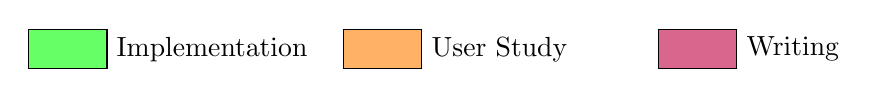
\begin{tikzpicture}[legend entry/.style={fill=#1,draw=black,rectangle,minimum width=1cm,minimum height=0.5cm}]
                \node[legend entry=green!60] at (0,0) {};
                \node[right] at (0.5,0) {Implementation};
                \node[legend entry=orange!60] at (4,0) {};
                \node[right] at (4.5,0) {User Study};
                \node[legend entry=purple!60] at (8,0) {};
                \node[right] at (8.5,0) {Writing};
            \end{tikzpicture}
            \caption{Schedule of my Master Thesis}
            \label{fig:time_shedule}
        \end{figure}
    \end{landscape}


\end{linenumbers}


\clearpage
\printglossary[type=\acronymtype]
\clearpage
\printbibliography



\end{document}
